\documentclass[conference]{IEEEtran}
\usepackage[english]{babel}
\usepackage[autostyle]{csquotes}
\usepackage{amsmath,amssymb,amsfonts}
\usepackage{algorithmic}
\usepackage{graphicx}
\graphicspath{{images/}}
\usepackage{textcomp}
\usepackage{xcolor}
\usepackage[outputdir=output]{minted}
%\usemintedstyle{autumn} % friendly, colorful
%\newminted{c}{mathescape, linenos, numbersep=5pt, gobble=0, frame=lines, framesep=2mm}
%\definecolor{background}{gray}{0.90}
%\newminted{bash}{bgcolor=background}
%\newminted{console}{bgcolor=background}
%\usemintedstyle[console]{bw}
\def\BibTeX{{\rm B\kern-.05em{\sc i\kern-.025em b}\kern-.08em
    T\kern-.1667em\lower.7ex\hbox{E}\kern-.125emX}}
\begin{document}

\title{Semantics Generation For A 3D Scene Using Raytracing and RenderMan}

\author{\IEEEauthorblockN{Mark Wesley Harris}
\IEEEauthorblockA{\textit{CS5800 Computer Graphics, Fall 2019} \\
\textit{University of Colorado Colorado Springs}\\
Colorado Springs, United States \\
wharris2@uccs.edu}}

\maketitle

\begin{abstract}
\end{abstract}

\section{Introduction}
\label{sec:introduction}


\section{Related Work}
\label{sec:related_work}
Schied \textit{et al.} \cite{spatiotemporal}
generated high quality outputs given very low quality input
frames. The inputs to the algorithm are rendered frames using one path-per-pixel global
illumination. As shown in Figure \ref{fig:spatiotemporal}, they are able to
transform very crude, noisy frames into production-grade outputs comparable to
the frames rendered at full resolution. Their algorithm is essentially a
multi-pass filter which the inputs are fed into, making it very fast and
reliable.

The proposed thesis work requires frame generation given scene data that has not yet been rendered,
while \cite{spatiotemporal} depends on the input of entire rendered frames.
However, there may be other components of the research that can be extracted.

\begin{figure}[htbp]
\centerline{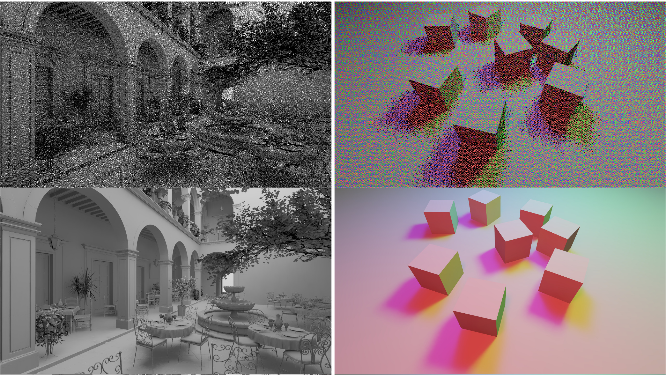
\includegraphics[width=8cm]{spatiotemporal.png}}
\caption{Example input and output frame of \cite{spatiotemporal}.}
\label{fig:spatiotemporal}
\end{figure}

\cite{backwards_raytrace}
\cite{arnold}
\cite{renderman}

\subsection{Architectural Overview}
\label{sec:architecture}
The proposed focus for this work is based off of the research presented in
\cite{pose_guided}.
See Figure \ref{fig:block_diagram} for a basic block diagram of the proposed architecture.
The most important component
is Generator I, which uses a combination of machine learning models to generate a
low resolution image containing global structures found in the
source data.

\begin{figure}[htbp]
\centerline{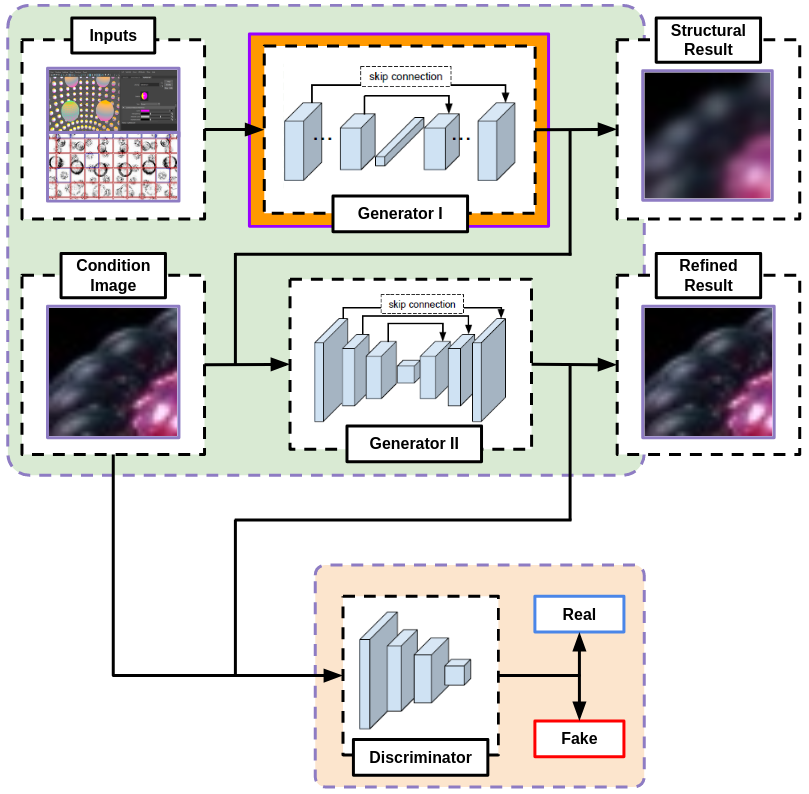
\includegraphics[width=8cm]{block_diagram.png}}
\caption{Block diagram for proposed architecture.}
\label{fig:block_diagram}
\end{figure}

\section{Proposed Work}
\label{sec:proposed_work}
Discussed in \cite{renderman_opengl} is a walkthrough comparison of OpenGL to RenderMan.
RenderMan documentation is found in \cite{renderman_docs}.
Raytracing walkthrough is found in \cite{raytrace_walkthrough}.

\subsection{Semester Plan}
\label{subsec:semester_plan}
\begin{enumerate}
\item \textbf{Environment Setup, \textit{9/8 -- 9/17}}
\begin{itemize}
\item Maya -- Source 3D animation and modeling software.
\item RenderMan -- Download and install. Integrate with Maya.
\end{itemize}
\item \textbf{Test Render Pipeline, \textit{}}
\begin{itemize}
\item Basic working scene -- Work from animation file used in \cite{thesis_harris}.
\item Basic working script -- Using RenderMan documentation \cite{renderman_docs}.
\end{itemize}
\item \textbf{Explore RenderMan, \textit{9/17 -- 10/1}}
\begin{itemize}
\item Program Raycasting -- Using OpenGL to RenderMan discussion \cite{renderman_opengl}
and Raytrace Walkthrough \cite{raytrace_walkthrough} as references.
\end{itemize}
\item \textbf{Export Object Semantics, \textit{10/8 -- 10/22}}
\begin{itemize}
\item Find objects associated with each pixel.
\item Export in a parsable format for ML processing.
\end{itemize}
\end{enumerate}

\section{Evaluation}
\label{sec:methods/evaluation}


\section{Conclusion}
\label{sec:conclusion}

\bibliographystyle{IEEEtran}
\bibliography{proposal}

%==========================================================
\end{document}
%==========================================================
